\chapter{\IfLanguageName{dutch}{Stand van zaken}{State of the art}}
\label{ch:stand-van-zaken}

% Tip: Begin elk hoofdstuk met een paragraaf inleiding die beschrijft hoe
% dit hoofdstuk past binnen het geheel van de bachelorproef. Geef in het
% bijzonder aan wat de link is met het vorige en volgende hoofdstuk.

% Pas na deze inleidende paragraaf komt de eerste sectiehoofding.

In dit hoofdstuk worden de verschillende termen die aan de InsurTech en Webscraping gebonden zijn uitvoerig besproken.

\section{InsurTech}

Allereerst wordt de term InsurTech verklaard.
InsurTech is een porte-manteauwoord van insurance en technology.
Concreet is dit het introduceren of gebruik maken van innovatieve technologie in de verzekeringswereld.
Deze innovatieve technologiën worden ontwikkeld door middel van het gebruik van apps, Big Data, machine learning, draagbare producten zoals smartwatches en andere transformatieve technologiën die processen betreffende de verzekeringswereld kunnen automatiseren of bevorderen. Deze bevorderingen kunnen gaan van 
De InsurTech is in principe een specialisatie van FinTech, ofwel Financial Technology.
Terwijl FinTech zich op alle financiële technologieën focust, beperkt de InsurTech zich tot die van de verzekeringswereld.
Een duidelijk verschil is dat de FinTech onder meer ook nog over technologie in banken gaat.

InsurTech is nog vrij nieuw, zo worden er regelmatig nieuwe toepassingen ontwikkeld die de efficiëntie van een verzekeringsbedrijf bevordert. Zo wijst een artikel van \textcite{Institute2020} erop dat de term is opgekomen rond 2010, toen de hoofdimplementatie eerder prijsvergelijkingen tussen verschillende verzekeringsmaatschappijen was. Tegenwoordig reiken de toepassingen van InsurTech veel verder dan alleen prijsvergelijkingen, zoals verzekeringsadvies bieden op basis van verzamelde data. Een ander artikel uit 2021 of \textcite{InsuranceCommissioners2021} toont aan dat InsurTech startups de voorbije decennia een geschatte 16,5 miljard dollar aan investeringen hebben verzameld en dat dit bedrag in de toekomst alleen maar zal groeien. Een literatuurstudie van \textcite{inproceedings} concludeert dat de verzekeringsmaatschappijen vooral kosten, in tijd en geld, verliezen door het analyseren van de risico’s die een klant loopt om zo de juiste verzekeringen aan te raden. Door InsurTech toepassingen is het beheren van verzekeringen en de klantencommunicatie niet alleen vergemakkelijkt, maar ook verbeterd. Wat webscraping en datamining betreft bestaat er reeds een grote variëteit aan technologie en tools. Er zal zowel voor een toepassing voor webscraping, als API gebruik gezocht worden bij het vinden van een toepassing die de klantenervaring kan bevorderen.

\subsection{De werking van verzekeringen}
Een verzekering wordt door \textcite{Trowbridge1975} omschreven als een risico-overdracht waarbij
een klant het risico overdraagt aan een verzekeringsmaatschappij in ruil voor een overeengekomen bedrag. 
Het doel van de klant in dat geval is de negatieve financiële gevolgen te beperken van een onzekere toekomstige gebeurtenis.
\graphicspath{ {./img/} }
\begin{figure}[H]
	\centering
	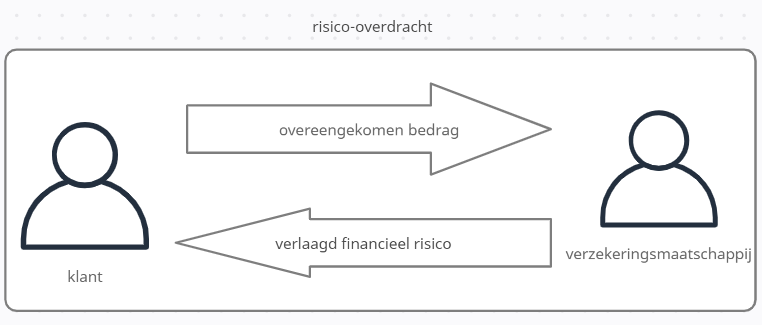
\includegraphics{creately_basic_verzekering}
	\caption{Verzekering visualisatie volgens \textcite{Trowbridge1975}}
\end{figure}
Een verzekering krijgt volgens \textcite{cortis2019insurtech} verder ook de taak en verantwoordelijkheid een inschatting te maken over welk bedrag opgesteld moet worden. Dit is afhankelijk van de grootte van het risico die de verzekeringsmaatschappij met zich meedraagt. Wanneer een klant zijn vergoeding opeist, wordt bij de verzekering een claim management proces opgesteld. Dit is opnieuw één van de processen waar tijd- en kost-efficiëntie een rol speelt.



\section{Webscraping}

Allereerst gaan we terug in de tijd, naar het ontstaan van webscraping. Webscraping dateert al van het begin van het World Wide Web, ontstaan in 1989, toen het internet voor het eerst werd geïntroduceerd. Nog geen 4 jaar later, in 1993, werd al voor het eerst de term “webscraping” gebruikt. Het jaar waarin een groep MIT (Massachusetts Institution of Technology) studenten als schoolproject de omvang van het internet probeerden in te schatten. Hun allereerste webscraper, de World Wide Web Crawler, werd de basis van vele andere webscrapers die nog in de toekomst zouden volgen. In datzelfde jaar werd alsook de allereerste zoekmachine op het internet uitgevonden door Jonathan Fletcher, de “vader van de zoekmachine”. Deze student aan de University of Sterling te Schotland ontwierp onbewust de voorloper van Google genaamd Jumpstation. \autocite{farholt2021less} Mettertijd is het gebruik van webscraping en de gebruikte toepassingen drastisch gewijzigd. Zo worden tegenwoordig webscrapers gebruikt om interactie van een gebruiker te simuleren om webpagina’s uit te testen vanuit het standpunt van de eindgebruiker.
Webscraping is reeds heel wat geëvolueerd, zo moet de technologie zich vaak aanpassen aan hoe webpagina’s eigenlijk opgebouwd zijn.
Webscraping is het extraheren en indexeren van data in webpagina’s en deze vervolgens opslaan in een tekstbestand of databank. Webpagina’s bestaan uit tekst die in verschillende formaten beschikbaar is: als gewone tekst, in tabellen, ... De simpelste vorm van webscraping het kopiëren en plakken van tekst. Het is de taak van een webscraper deze data automatisch uit te lezen en te indexeren. Het crawlen of scrapingsproces op het internet bestaat er allereerst uit alle gewenste data uit te lezen om deze vervolgens in een gepast leesbaar formaat te structureren.\autocite{zhao2017web} Hoofdzakelijk wordt dit gebruikt om repetitieve taken te versnellen, zoals iedere subtitel van een pagina kopiëren en plakken. Het uitlezen kan op verschillende manieren gebeuren, afhankelijk van de desbetreffende webpagina. Echter is het niet hoofdzakelijk nodig altijd webscraping toe te passen. Soms beschikt de webpagina of service over een API, een acroniem voor Application Programming Interface. Dit is een set van functies en procedures gebruikt die één of meerdere taken vervuld met als doel door software gebruikt te worden. Dit maakt het voor programmeurs makkelijker en efficiënter om net de data die men nodig heeft uit de pagina te halen zonder overbodige data ook nog in te laden. Performantiegewijs heeft het gebruik van API’s op webpagina’s of services duidelijk de voorkeur. \autocite{10.2307/251584}
Abstract kan het gebruik van webscraping vanalles inhouden. Kleinschalig kan dit gaan over het monitoren van real-time data met behulp van polling, wat een detectiesysteem kan inhouden die aanpassingen op websites detecteert. Tot grootschalig het voortdurend uitlezen van website data om een zoekmachine mee te bouwen. Zo kan Google of Bing aanzien worden als één grote webscraper, gebruikt om het internet uit te mappen. \autocite{snyder2003web}

\begin{figure}[bh]
	\centering
	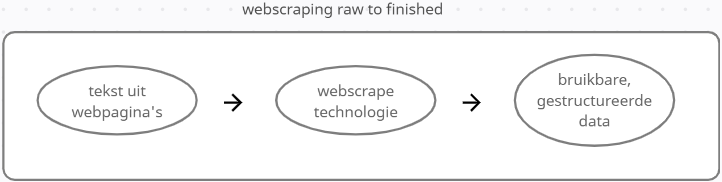
\includegraphics{webscraping_cycle}
	\caption{webscraping structuur}
\end{figure}

\subsection{Populaire Webscrapers}

% TODO leg uit waarom er gekozen werd voor enkel Selenium en puppeteer uit te leggen dmv populariteit
Een recent onderzoek duidt aan dat Selenium en Puppeteer tussen de populaire webscrapers zitten. (Saurkar e.a., 2018)


\subsection{Puppeteer}

% TODO vul aan wat Puppeteer is
Puppeteer

\subsection{Selenium}

Selenium is een web-UI testing library, wat wil zeggen dat de library geschikt is voor testdoeleinden. Selenium is echter niet beperkt tot deze doeleinden. Het is een set van verschillende software tools die elk een verschillende aanpak hebben om geautomatiseerde testen te ondersteunen. Het geautomatiseerd testen is de techniek van het automatiseren van de uitvoerings van testgevallen met behulp van gespecialiseerde software. Het feit dat deze library ondersteund wordt in verschillende webbrowsers maakt de library zeer toegankelijk.

\begin{figure}[bh]
	\centering
	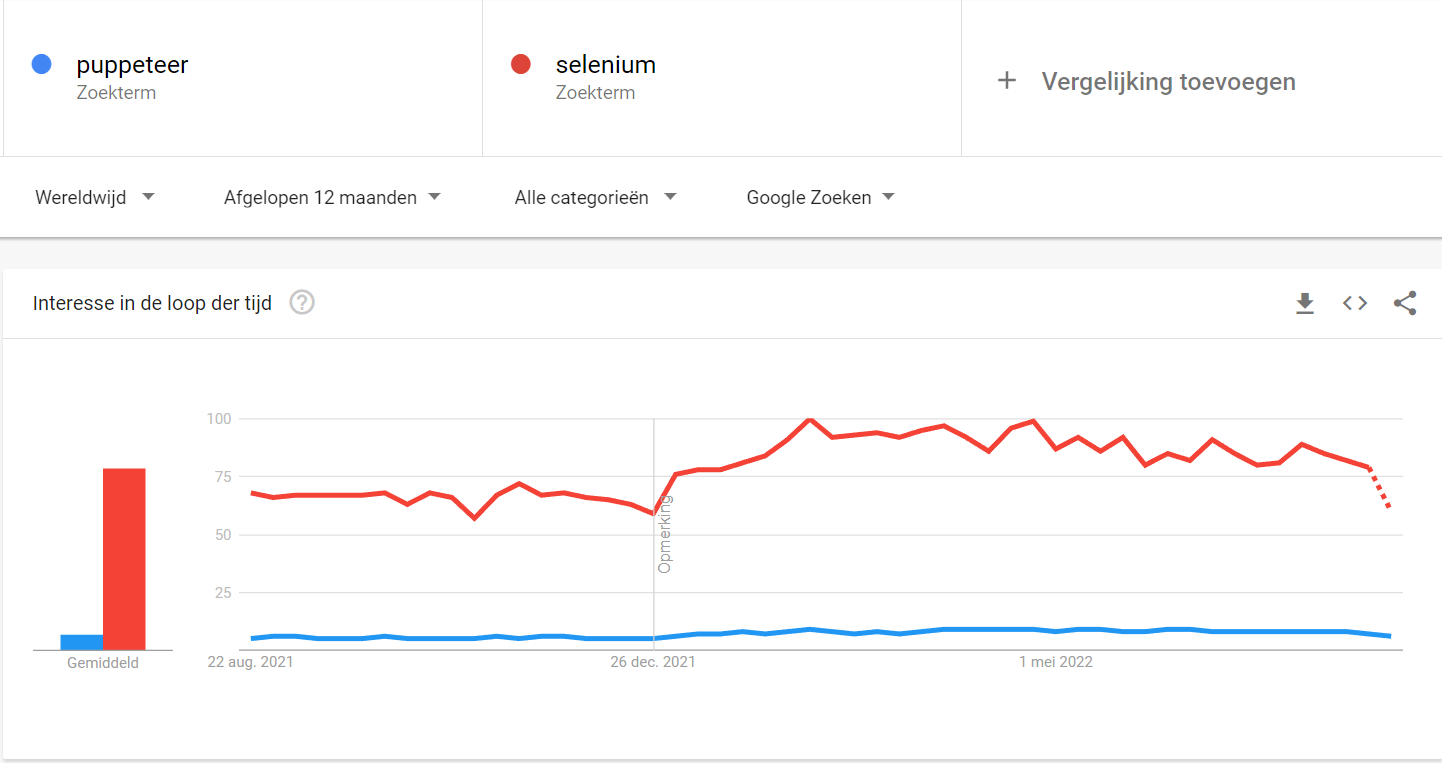
\includegraphics[width=\paperwidth, height=\textheight, keepaspectratio]{selenium_puppeteer_google_trends}
	\caption{Vergelijking Selenium vs Puppeteer op \href{https://trends.google.com/trends}{Google Trends}}
\end{figure}

\section{Databanken}

Er worden steeds meer gegevens verzameld en gebruikt, mede door middel van hierboven beschreven webscrapers. Als gevolg daarvan zijn databanken belangrijker dan ooit.
Om  data op te slaan is nood aan gestructureerde opslag, zodat de inhoud ervan makkelijk toegankelijk en beheerbaar is. 

Opslag van data in een soort databanken bestaat al enkele millenia. De Egyptenaren zouden de voorvaders kunnen genoemd worden in het opslaan van data. Ze hielden informatie bij door in stenen te kerven of op dierenhuiden te schrijven. Flash forward naar de 21e eeuw en er zijn al heel wat nieuwe modernere methoden om data op te slaan, voornamelijk op computers met gebruik van een databank.
Een databank is een collectie van deze data, waarin data records of bestanden door een databank manager worden beheerd. \autocite{obenshain_2004} Databanken worden gebruikt om gegevens efficiënt op te slaan en op verzoek alle data of een delen ervan terug te bezorgen. Databank tools bevatten gebruikelijk een zoekfunctie waarbij vragen zoals "Wie heeft het voorbije jaar een verzekeringscontract afgesloten?" kunnen beantwoord worden. Deze databanken worden voornamelijk gebruikt binnen grote mainframe systemen, alsook kleinere systemen of persoonlijke computers. Het is nutteloos als ze in een database zitten en niets doen. Er wordt gebruik gemaakt van software om er iets van te maken. Software formatteert deze opgeslagen data en structureert ze op een manier die zinvol is en ons in staat stelt weloverwogen beslissingen te nemen.

% TODO: voeg databank figure toe met fields en records voorbeeld

\section{Datamining}

Datamining is een multidisciplinair gebied dat statistiek, databanktechnologie, patroonherkenning, machine learning, gegevensvisualisatie en expertise in systemen omvat.
Wanneer een onderzoek werkt met grote datasets, is het manueel nagaan van verbanden ingewikkeld en heeft de data dus als vereiste automatisch gecontroleerd te worden.
Datamining bestaat uit het onderzoeken van bestaande data uit grote bestaande databanken, met als doel nieuwe data te genereren. Datamining is eerder waardevol voor gecompliceerdere zoektermen, zoals "Welk verband kan gevonden worden tussen de verzekeringscontracten die afgesloten werden het voorbije jaar?".
Op zichzelf is datamining een proces waar, in een grote set data, onderzoek wordt gedaan naar nuttige, relevante data. Het vinden van patronen, algoritmes en afwijkingen in deze grote set data moeten hierbij helpen. Het doel van de datamining techniek is om net ongekende patronen te vinden in de set data om deze vervolgens met elkaar te kunnen linken en structureren. Dit kan dan een antwoord bieden op business gerelateerde vragen die te tijd consumerend zijn om zelf op te lossen. \autocite{osman2019data} In detail kan dit logisch proces is onderverdeeld in 2 delen: het wetenschappelijke en het commerciële. Voornamelijk zijn toepassingen die het dataminen bevorderen in de InsurTech voornamelijk gefocust op het commerciële. \autocite{hand2007principles}

\subsection{Datamining proces}

Om datamining om te zetten in praktijk, namelijk van het extraheren van data tot het visualiseren ervan, worden een aantal stappen ondernomen.


\section{Webscraping vs Datamining}

Nu voorgaande termen onderling zijn besproken, wordt het verschil of de samenhang van beiden besproken. In het kort werd webscraping eerder omschreven als een data ophalen. Terwijl webscraping eerder het ophalen van data is en formatteren doet het geen analyse of dataprocessing. Het is net de datamining die de opgehaalde data zal verrijken en hieruit conclusies, verbanden en verschillen uit zal halen. In feite kan web scraping dus gebruikt worden om datasets te creeëren waarop datamining wordt toegepast. Deze beiden vullen elkaar dus aan.


\section{Tools}

Bij webscraping is het belangrijk om de juiste tool te vinden die voldoet aan jouw benodigdheden.
Zo is het bij dit onderzoek de bedoeling enkel webscrapers te gebruiken die draaien op de programmeertaal Python, dus is \href{https://nutch.apache.org}{Apache Nutch} bijvoorbeeld al niet van toepassing. Zo zijn er nog vele andere webscraping tools die \textcite{Sirisuriya2015} aanhaalt in haar studie.
Bij een recent onderzoek naar de meestgebruikte tools in Python kwamen Selenium en Puppeteer als één van de populairste uit de bus. \autocite{Saurkar2018}
Vandaar zal ook bij dit onderzoek deze tools gebruikt worden. Deze maken gebruik van webautomatie om hun taak te vervullen.

\section{InsurTech mogelijkheden}

Niet alleen de FinTech heeft reeds doorbraken gehad op technologisch vlak die als een ware revolutie lijken. Eind de jaren 1900 werd de bankautomaat, die het mogelijk maakte na sluiting van de bank nog steeds geld af te halen, in België geïntroduceerd. Hoewel dit echter al een enorme stap in de digitale revolutie was, werd 2 decennia later de mobiele betalingstechnologie een noviteit. \autocite{agarwal2020real} Deze voorbeelden van mogelijkheden binnen de FinTech zijn niet de enige die efficiëntie van het bankieren bevorderen. Echter ligt de focus bij dit onderzoek op de mogelijkheden die reeds bestaan en nog kunnen bestaan in de InsurTech. De twee hoofdgebieden waar conservatieve en moderne verzekeringsmaatschappijen gerelateerd zijn betreffen data en consumenten. Door gebruik te maken van InsurTech mogelijkheden kunnen conservatieve verzekeraars nieuwe producten en diensten aanbieden, de verzekeringsdekking uitbreiden tot voorheen onderverzekerde marktgroepen, de verwerking van claims stroomlijnen, de transactiekosten verlagen, en zorgen voor een betere risicobeoordeling en -bewaking. Door de technologische ontwrichting staan de verzekeringsmaatschappijen steeds meer onder druk om hun klantgerichte procedures te moderniseren en te innoveren. De digitale knowhow van insurtech-bedrijven, waarvan de aanwezigheid eerder als een kans dan als een bedreiging moet worden gezien, zou op dit gebied een nuttige hulp kunnen zijn. Welke knowhow dit precies is en hoe deze wordt geïmplementeerd is deel van het onderzoek dat volgt. \autocite{koprivica2018insurtech}
